\chapter{Аналитический раздел}

% В данном разделе приводятся анализ предметной области. Также рассматривается обзор методов обнаружения фальсификаций в изображении. Сформулируются критерии их сраванения и приводится сравнительный анализ рассмотренных методов. Также в этом разделе представляется формализованная постановка задачи в виде IDEF0-диаграммы.

\section{Фальсификация изображений и задача её обнаружения}

\subsection{Понятие фальсификации изображений}

Под фальсификацией (подделкой) цифровых изображений понимается процесс преднамеренного внесения изменений в исходное изображение с целью искажения его визуального содержания или передаваемого смысла. В отличие от стандартной обработки изображений (коррекция яркости, контраста, цветокоррекция, шумоподавление или ретушь в художественных целях), фальсификация всегда преследует цель ввести зрителя в заблуждение, создать ложное представление о реальности, что может использоваться как в личных, так и в профессиональных или политических целях \cite{1}.

С развитием доступных инструментов редактирования (Adobe Photoshop, GIMP) и особенно методов искусственного интеллекта возможности создания высококачественных подделок значительно возросли. Современные генеративные модели, позволяют генерировать или модифицировать изображения с уровнем реализма, который часто невозможно отличить невооружённым глазом. В связи с этим задача обнаружения фальсификаций становится особенно актуальной в областях журналистики, криминалистики и социальных медиа \cite{2}.

В современной литературе по компьютерному зрению принято выделять несколько основных типов фальсификации изображений\cite{3}.

\begin{itemize}[label= ---]

	\item Копирование-вставка (англ. copy-move) --- фрагмент изображения копируется и вставляется в другую область того же изображения, часто для сокрытия объектов или их дублирования.

	\item Вставка объектов из другого изображения (англ. splicing) --- часть одного изображения переносится в другое, создавая сцену, которой не существовало в действительности.

	\item Ретуширование (англ. inpainting) --- удаление или замена элементов с помощью заполнения области (удаление теней, людей, артефактов, ...).

	\item Генерация полностью синтетических изображений --- создание изображений с нуля с использованием генеративно-состязательных сетей (GAN) или диффузионных моделей.

	\item Deepfake --- замена лица или мимики человека на видео и изображениях с использованием нейросетевых методов.
\end{itemize}

Ниже, на рисунке \ref{1-fake}, представлены примеры фальсификаций изображений типа копирование-вставка.

\captionsetup{justification=centering,singlelinecheck=off}
\begin{figure}[h!]
	\centering
		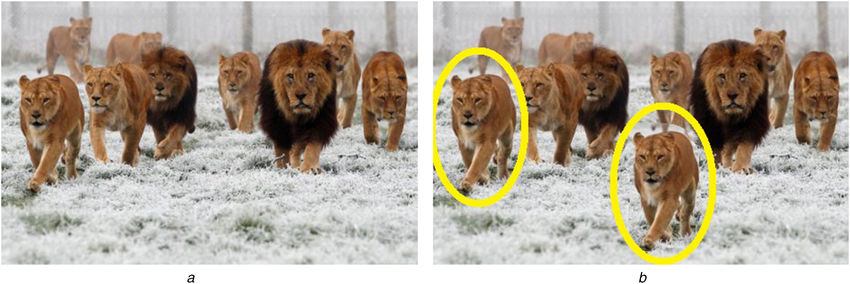
\includegraphics[,scale=0.5]{./img/example.png}
		\caption{Пример фальсификаций изображений типа копирование-вставка.}  
		\label{1-fake}
\end{figure}

Цифровая фальсификация оставляет определённые статистические и семантические следы. Например, при копировании-вставке возникает повторяющаяся структура блоков, при вставке --- нарушение согласованности шума датчика или освещения, а при ретушировании --- аномалии в частотной области (артефакты сглаживания, некорректное сохранение JPEG)\cite{4}.

Важно отметить, что понятие фальсификации не включает в себя такие изменения, как сжатие с потерями, масштабирование или поворот, если они не направлены на введение в заблуждение зрителя. Однако в реальных условиях поддельное изображение часто подвергается дополнительным операциям (JPEG-сжатие, изменение размера, фильтрация), что усложняет его обнаружение\cite{5}.

Таким образом, для обнаружения фальсифицированного фрагмента необходимо учитывать множество потенциальных аномалий на различных уровнях представления изображения: от пиксельного до семантического.

\subsection{Основные трудности и требования к методам обнаружения}

Задача обнаружения фальсифицированного фрагмента на изображении относится к классу задач пассивной судебной экспертизы изображений. В отличие от активных методов (цифровая подпись, водяные знаки), пассивные методы не требуют предварительного внедрения вспомогательной информации, однако сталкиваются с рядом принципиальных трудностей, обусловленных как свойствами самих изображений, так и действиями злоумышленника\cite{6}.

К числу основных трудностей относятся.

\begin{enumerate}
	\item Отсутствие эталонного («чистого») изображения. В большинстве практических сценариев (например, при проверке фотографий в СМИ или на интернет-платформах) исходное неизменённое изображение недоступно. Поэтому метод должен выявлять аномалии исключительно на основе статистических и семантических характеристик самого анализируемого файла.
	
	\item Разнообразие типов фальсификаций. Как отмечалось в п. 1.1.1, подделки могут быть выполнены методами copy-move, splicing, inpainting, deepfake и др. Каждый тип оставляет различные следы: повторяющиеся блоки, несоответствие шума сенсора, артефакты интерполяции или генеративные контуры. Универсальный метод должен быть устойчивым к нескольким типам подделок \cite{7}.
	
	\item Сокрытие следов подделки послеоперационной обработкой. Злоумышленник может применять к поддельному изображению сжатие JPEG, масштабирование, добавление шума, медианную фильтрацию или размытие. Эти манипуляции намеренно затрудняют обнаружение артефактов, разрушая статистические аномалии, внесённые в момент фальсификации.
	
	\item Разнородность исходных изображений. Метод не должен полагаться на фиксированные характеристики (размер, разрешение, цветовое пространство, модель камеры), так как изображения в реальных условиях поступают из самых разных источников \cite{8}. Это требует инвариантности к разрешению, коэффициенту сжатия и уровню шума.
	
	\item Вычислительная сложность и требования к ресурсам и времени. Применение метода в потоковых системах (социальные сети, новостные агрегаторы) требует быстрой обработки (миллисекунды на изображение) и работы с большими объёмами данных. Слишком ресурсоёмкие модели неприменимы в реальном времени.

	\item Отсутствие крупных универсальных размеченных наборов данных. Обучение методов на основе глубокого обучения требует большого количества подлинных и фальсифицированных изображений с пиксельной разметкой подделанных областей. Существующие датасеты различаются по типам подделок, размерам и условиям создания, что затрудняет сравнение и обобщение.
\end{enumerate}

В связи с перечисленными трудностями к современным методам обнаружения фальсифицированного фрагмента предъявляются следующие требования \cite{9}:

\begin{itemize}[label = ---]
	\item Высокая точность: метод должен обеспечивать высокие значения метрик IoU, F1-меры и точности классификации пикселей на тестовых наборах, сбалансированных по типам подделок.
	
	\item Устойчивость к постобработке: метод должен сохранять работоспособность после сжатия JPEG, изменения размера, добавления шума и других типов постобработки.
	
	\item Обобщающая способность: обученная модель должна корректно работать на изображениях, взятых из датасетов, не участвовавших в обучении, и на неизвестных типах подделок.
	
	\item Вычислительная эффективность: время детекции одного изображения должно быть сопоставимо с временем его загрузки или публикации.
	
	\item Локализация фрагмента: метод должен не только выносить бинарное решение, но и выдавать карту локализации с указанием границ изменённой области (пиксельная маска).
	
	\item Инвариантность к изображению: метод не должен зависеть от конкретной модели камеры, формата и цветовой схемы (RGB, YCbCr).
\end{itemize}

Таким образом, разработка практического метода обнаружения фальсифицированного фрагмента представляет собой сложную многокритериальную задачу, требующую компромисса между точностью, устойчивостью и скоростью работы.

\section{Методы обнаружения фальсифицированного фрагмента на изображении}

В настоящее время существует множество подходов к решению задачи обнаружения фальсифицированных фрагментов изображений. Все методы можно условно разделить на три основные группы: методы на основе анализа целостности изображений, методы на основе поиска ключевых точек и методы на основе сверточных нейронных сетей. Каждый из них имеет свои сильные и слабые стороны, область применимости и уровень эффективности.

\subsection{Методы на основе анализа целостности изображений}

Методы обнаружения фальсифицированного фрагмента на основе анализа целостности изображений опираются на предположение, что любая модификация исходного изображения нарушает определённые статистические закономерности, присущие естественным изображениям. В отличие от методов поиска ключевых точек, которые ориентированы преимущественно на выявление фальсификации типа копирование-вставка, подходы на основе целостности анализируют непротиворечивость таких физически обоснованных характеристик, как шум датчика (PRNU), артефакты двойного сжатия JPEG и корреляции, вносимые интерполяцией цветных фильтров (CFA). Каждый из этих трёх методов имеет собственную область эффективности и ограничения. На практике эти методы часто применяются в комплексе: например, сначала выполняется анализ PRNU для грубой локализации подозрительных областей, а затем уточнение с помощью CFA-интерполяции. Такой многоэтапный подход позволяет снизить количество ложных срабатываний \cite{2}.

Принципиальным преимуществом методов анализа целостности является их независимость от наличия обучающей выборки, что характерно для нейросетевых подходов. Они основаны на фундаментальных физических свойствах процесса формирования цифрового изображения, которые трудно подделать или полностью скрыть без значительной деградации визуального качества. Это делает их особенно ценными в сценариях судебной экспертизы, где требуется предоставить объяснимое и юридически обоснованное заключение о подлинности изображения. Однако, каждый из методов имеет существенные ограничения, связанные с чувствительностью к постобработке, необходимостью априорной информации об устройстве съёмки и сложностью точной локализации границ фальсификации.

\textbf{Метод на основе анализа шума датчика (PRNU)}

Каждая цифровая камера оставляет уникальный «отпечаток» --- фотоотклик неравномерности (photo-response non-uniformity, PRNU), возникающий из-за неоднородной чувствительности пикселей \cite{4}. При вставке фрагмента из другого изображения (splicing) в подделанной области нарушается согласованность PRNU: появляется шум другой камеры или его отсутствие. Метод вычисляет PRNU анализируемого изображения (обычно с помощью вейвлет-фильтрации или использования фильтра высоких частот) и оценивает его корреляцию с эталонным шумом предполагаемой камеры. Если фрагмент изображения имеет статистически значимое расхождение в структуре шума, это свидетельствует о фальсификации. 

Физическая природа PRNU обусловлена несовершенством полупроводниковой технологии производства матриц: каждый пиксель имеет слегка различную чувствительность к падающему свету, что создаёт уникальный пространственный паттерн, который можно рассматривать как цифровой отпечаток пальца камеры. Этот паттерн остаётся стабильным для данной камеры на протяжении всего срока её службы и не зависит от снимаемой сцены. Для выделения PRNU из изображения применяются методы подавления контентной составляющей, чаще всего с использованием вейвлет-преобразования или фильтрации в частотной области. Наиболее распространённым подходом является использование фильтра высоких частот, который извлекает компоненту шума, содержащую как PRNU, так и другие виды шумов. Для повышения отношения сигнал-шум обычно используют усреднение по нескольким изображениям, снятым одной камерой, чтобы подавить случайную составляющую и выделить стационарный PRNU-компонент.

Ниже, на рисунке \ref{1-prnu}, представлена схема работы метода на основе анализа шума датчика (PRNU).

\captionsetup{justification=centering,singlelinecheck=off}
\begin{figure}[h!]
	\centering
		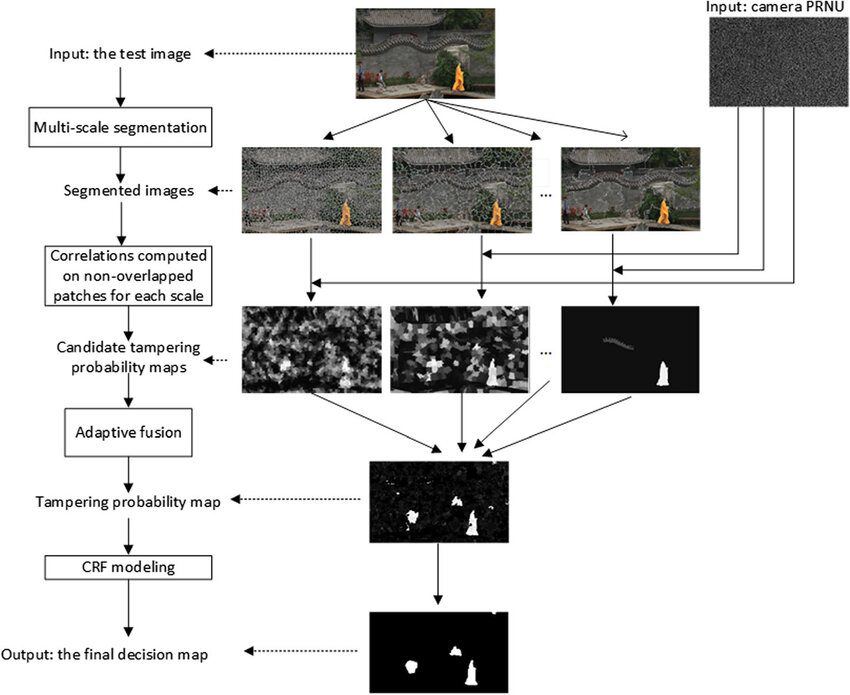
\includegraphics[,scale=0.5]{./img/prnu.png}
		\caption{Схема работы метода на основе анализа шума датчика.}  
		\label{1-prnu}
\end{figure}

В работе \cite{10} также показано, что эффективность PRNU-анализа резко падает, если фальсифицированный фрагмент был предварительно обесцвечен или подвергнут нелинейной гамма-коррекции. Для повышения робастности исследователи предлагают использовать вейвлет-преобразование Хаара, которое сохраняет высокочастотную составляющую шума даже при умеренном сжатии. Однако при коэффициенте качества JPEG ниже 75\% PRNU-следы становятся практически неразличимыми. Кроме того, практическое применение метода требует, чтобы на изображении была как минимум одна область с заведомо неизменённым шумом. Такую область часто выделяют вручную или с помощью алгоритмов поиска однородных текстур. Без этого эталонного фрагмента корреляционный анализ теряет смысл. На практике PRNU-метод наиболее полезен при расследовании единичных целенаправленных фальсификаций, где камера-источник может быть изъята и исследована. В потоковой обработке интернет-изображений практически не применяется из-за отсутствия эталонных шумов.

Несмотря на свою теоретическую привлекательность, PRNU-анализ сталкивается с рядом серьёзных практических ограничений. Во-первых, для вычисления эталонного PRNU камеры требуется доступ к самой камере или серии изображений, снятых ею, что часто невозможно в реальных сценариях расследования. Во-вторых, даже при наличии эталонного PRNU, корреляционный анализ даёт лишь вероятность того, что фрагмент был снят другой камерой, но не позволяет точно определить границы вставки без дополнительных методов сегментации. В-третьих, злоумышленник может сознательно применить к вставленному фрагменту обработку, разрушающую структуру шума: например, повторное сжатие с последующим добавлением синтетического шума или применение дебайзеринга с другой моделью демозаики. Это позволяет эффективно маскировать несоответствие PRNU, сохраняя при этом приемлемое визуальное качество подделки. Кроме того, метод крайне чувствителен к масштабированию: изменение размера фрагмента разрушает пространственную структуру PRNU, делая корреляционный анализ невозможным.

\textbf{Метод на основе двойного сжатия JPEG (Double JPEG)}

Большинство цифровых изображений сохраняются в формате JPEG с потерями. Если злоумышленник редактирует изображение и сохраняет его повторно, возникает так называемое двойное сжатие с возможно разными таблицами квантования. При этом гистограмма коэффициентов дискретного косинусного преобразования (DCT) для отдельных частотных полос приобретает характерные периодические пики. Метод анализирует гистограммы DCT-коэффициентов и выявляет наличие двух различных стадий квантования. В наиболее развитой форме метод не только определяет факт двойного сжатия, но и оценивает параметры первого сжатия \cite{11}. Достоинства: работает без какой-либо априорной информации об исходной камере, устойчив к умеренным атакам. Недостатки: метод даёт в основном бинарный ответ и плохо локализует точную область вставки; кроме того, если злоумышленник сохранил подделку без сжатия (в формате PNG) или использовал тот же коэффициент качества, двойное сжатие может быть не обнаружено.

Основой метода является анализ гистограмм квантованных DCT-коэффициентов для каждого из 64 частотных каналов (8×8 блоков). При однократном сжатии гистограммы имеют характерное распределение, близкое к обобщённому гауссовскому. При повторном сжатии с другими параметрами квантования в гистограммах возникают периодические артефакты — так называемые "столбчатые" выбросы, обусловленные тем, что значения, кратные шагу квантования второго сжатия, оказываются перераспределены по отношению к значениям, кратным шагу первого квантования. Эти выбросы можно выявить с помощью спектрального анализа гистограмм: например, вычисляя дискретное преобразование Фурье (DFT) от гистограммы и анализируя наличие характерных пиков. Современные варианты метода позволяют не только бинарно классифицировать изображение как подвергшееся двойному сжатию, но и оценивать параметры первого квантования, что может дать важную информацию об истории обработки изображения.

Ниже, на рисунке \ref{1-doublejpeg}, представлена гистограмма DCT исходного и сжатого изображений.

\captionsetup{justification=centering,singlelinecheck=off}
\begin{figure}[h!]
	\centering
		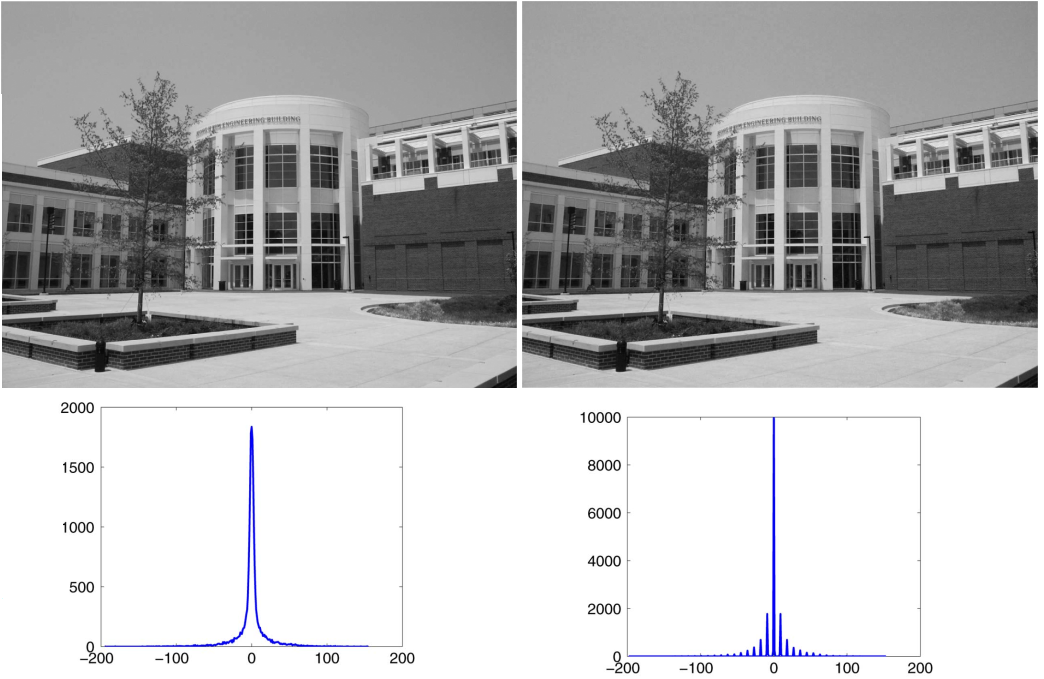
\includegraphics[,scale=0.5]{./img/doublejpeg.png}
		\caption{Гистограмма DCT исходного и сжатого изображений.}  
		\label{1-doublejpeg}
\end{figure}

Важным уточнением является то, что метод двойного сжатия эффективен только для подделок, которые были сохранены в JPEG хотя бы один раз после редактирования. Если оригинал был в формате без потерь, а фальсификация тоже сохранена без потерь, то DCT-гистограммы не покажут аномалий. Для улучшения локализации применяется скользящее окно фиксированного размера. Окно последовательно перемещается по изображению, и для каждой позиции вычисляется вероятность двойного сжатия. Области, где эта вероятность превышает порог, объединяются в итоговую карту подозрительных фрагментов. Такой подход, хотя и вычислительно затратен, позволяет очертить границы вставки с точностью до размера окна. Кроме того, устойчивость метода можно повысить, анализируя не только гистограммы, но и корреляции между DCT-коэффициентами соседних блоков. В подделанных областях эти корреляции часто нарушаются из-за того, что один блок мог быть сжат с одними параметрами, а соседний --- с другими. Данный приём, известный как «анализ блоковой когерентности», даёт хорошие результаты даже при повторном сжатии с тем же коэффициентом качества.

\textbf{Метод на основе анализа интерполяции цветных фильтров (CFA)}

Большинство цифровых камер используют матрицу цветных фильтров Байера, где каждый пиксель регистрирует только один цветовой канал (зелёный, красный или синий), а недостающие цветовые значения восстанавливаются с помощью демозаики. Процесс интерполяции вносит корреляции между соседними пикселями и между цветовыми каналами. При вставке фрагмента из другого изображения или при ретушировании локальная структура CFA-интерполяции нарушается, так как вставленная область имеет свою историю обработки. Метод моделирует ожидаемый процесс интерполяции для данной модели камеры или строит универсальную модель и вычисляет ошибку предсказания пикселя по соседним. В областях, где CFA-интерполяция нарушена, ошибка предсказания статистически значимо выше. Достоинства метода: возможность локализации подделки на уровне пикселей без необходимости знать эталонный PRNU. Недостатки: высокая чувствительность к сжатию JPEG, а также к масштабированию. Метод эффективен только для изображений, поступивших напрямую с камеры и сохранённых в формате без потерь или с минимальным сжатием \cite{12}.

Матрица Байера — это наиболее распространённый тип цветного фильтра, используемый в подавляющем большинстве цифровых камер. На каждом пикселе регистрируется только один цвет: зелёный (50\% пикселей), красный (25\%) или синий (25\%). Процесс демозаики восстанавливает два недостающих цветовых канала для каждого пикселя, используя интерполяцию значений соседних пикселей. Существует множество алгоритмов демозаики, от простой билинейной интерполяции до сложных адаптивных методов, учитывающих направление градиентов и текстуру. Независимо от конкретного алгоритма, процесс интерполяции вносит в изображение характерные корреляционные структуры, которые могут быть смоделированы. Если вставленный фрагмент был снят другой камерой или прошёл через иной процесс демозаики (например, через интерполяцию в графическом редакторе), то эти корреляции нарушаются, и ошибка предсказания (разница между предсказанным и реальным значением недостающего цветового канала) становится аномально высокой именно в области вставки.

Ниже, на рисунке \ref{1-cfa}, представлены исходное изображение и изображение, обработанное с помощью CFA. 

\captionsetup{justification=centering,singlelinecheck=off}
\begin{figure}[h!]
	\centering
		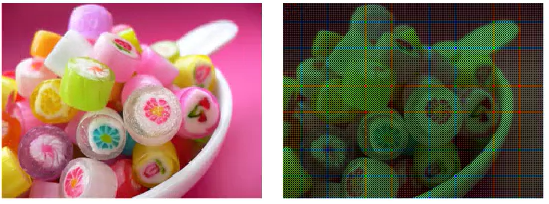
\includegraphics[,scale=1.0]{./img/cfa.png}
		\caption{Исходное изображение и изображение, обработанное с помощью CFA.}  
		\label{1-cfa}
\end{figure}

На практике CFA-метод часто реализуют через обучение небольшой нейронной сети предсказывать зелёный канал по красному и синему. Такую сеть обучают на заведомо подлинных изображениях, снятых различными камерами. При тестировании для каждого пикселя вычисляется ошибка предсказания; области с аномально высокой ошибкой маркируются как потенциально поддельные. Такой подход не требует явного задания модели интерполяции и частично компенсирует разницу между камерами разных производителей. Однако главное ограничение CFA-метода остаётся неизменным: он практически неработоспособен после сжатия JPEG с качеством ниже 90\%. Даже небольшое сжатие разрушает тонкие корреляции, внесённые демозаикой. Более того, если поддельный фрагмент был предварительно масштабирован или повёрнут, то его собственная CFA-интерполяция уже не соответствует исходной сетке Байера, и метод может дать ложное срабатывание даже на подлинной области.

Важным направлением развития CFA-методов является анализ не только ошибки предсказания отдельного пикселя, но и пространственных паттернов ошибки, которые могут выявлять характерные артефакты, свойственные конкретным алгоритмам демозаики. Также активно исследуются комбинированные подходы, объединяющие CFA-анализ с другими методами целостности (PRNU и Double JPEG) для повышения робастности к постобработке и увеличения точности локализации. Однако, несмотря на все усовершенствования, фундаментальное ограничение CFA-метода — его крайняя чувствительность к сжатию с потерями — остаётся серьёзным препятствием для его применения в условиях анализа изображений из интернета, где большинство файлов хранятся и передаются в сжатом формате JPEG с коэффициентом качества 70-80\%.

\subsection{Методы поиска ключевых точек}

Методы обнаружения фальсификации на основе поиска ключевых точек (англ. keypoint-based methods) являются одним из наиболее эффективных подходов для выявления фальсификации типа «копирование-вставка». Основная идея заключается в том, что при копировании фрагмента изображения и вставке его в другое место того же изображения в подделке появляются две или более области с идентичным или очень похожим содержанием. Ключевые точки представляют собой локальные особенности, инвариантные к масштабу, повороту и частично к изменению освещения, что позволяет обнаруживать дублированные фрагменты даже после их геометрического преобразования \cite{14}. Наибольшее распространение в задачах криминалистики изображений получили масштабно-инвариантное преобразование признаков (англ. Scale-Invariant Feature Transform, SIFT) и устойчивые ускоренные признаки (англ. Speeded-Up Robust Features, SURF) \cite{15}.

Математической основой инвариантности ключевых точек является построение масштабного пространства, в котором изображение свёртывается с гауссовым ядром при различных значениях параметра σ. Это позволяет представить изображение в виде пирамиды, где каждый последующий уровень соответствует уменьшенному масштабу или увеличенному размытию. Ключевые точки локализуются как экстремумы разности гауссовых функций в этом трёхмерном пространстве координат и масштаба. Такое представление обеспечивает инвариантность к масштабированию и повороту, поскольку ориентация ключевой точки определяется по гистограмме градиентов в её окрестности, что позволяет нормализовать дескриптор относительно преобладающего направления. Этот математический аппарат делает SIFT и SURF устойчивыми к геометрическим преобразованиям, которые часто применяются злоумышленниками для маскировки копирования.

\textbf{Метод SIFT}

Дескриптор SIFT, предложенный Лоу в 2004 году, стал золотым стандартом для обнаружения фальсификации типа копирование-вставка\cite{13}. Алгоритм включает следующие этапы: построение масштабного пространства, локализацию экстремумов разности гауссиа, отбраковку низкоконтрастных и граничных точек, назначение ориентации на основе градиентов и формирование 128-мерного дескриптора для каждой ключевой точки. При обнаружении подделки вычисляются SIFT-дескрипторы для всего изображения, затем выполняется их попарное сравнение (с использованием отношения расстояний до ближайшего и второго ближайшего соседа). Пары ключевых точек с высокой степенью совпадения дескрипторов группируются в кластеры с помощью алгоритмов иерархической кластеризации или DBSCAN, после чего для каждой группы строится ограничивающий прямоугольник или точный контур подозрительной области\cite{16}. SIFT демонстрирует высокую устойчивость к повороту, масштабированию и небольшому изменению перспективы, а также к сжатию JPEG при коэффициентах качества выше 70\%. Однако его вычислительная сложность относительно высока: извлечение дескрипторов и особенно их попарное сравнение может занимать несколько секунд на изображении среднего разрешения \cite{17}.

Глубокое понимание этапов алгоритма SIFT позволяет оценить как его сильные стороны, так и критические точки уязвимости. При построении масштабного пространства используется пирамида октав, каждая из которых состоит из нескольких уровней с различной степенью сглаживания. Локализация экстремумов разности гауссовых функций производится путём сравнения каждого пикселя с 26 соседями (8 в текущем масштабе + 9 в предыдущем + 9 в следующем), что обеспечивает высокую точность детектирования характерных точек. Этап отбраковки низкоконтрастных точек основан на анализе второй производной в экстремуме: если значение функции в точке меньше некоторого порога, точка считается неустойчивой и удаляется. Граничные точки, которые плохо локализуются из-за эффекта «края», отсеиваются с помощью анализа кривизны собственных значений матрицы Гессе. Назначение ориентации осуществляется построением гистограммы направлений градиентов в окрестности точки, где пик гистограммы определяет доминирующее направление, а дополнительные пики (если они значимы) создают несколько ключевых точек с разными ориентациями для одного местоположения. Итоговый 128-мерный дескриптор формируется путём разделения окрестности точки на блоки 4×4, для каждого из которых вычисляется гистограмма градиентов по 8 направлениям, что даёт 4×4×8 = 128 измерений. Такое избыточное представление обеспечивает высокую различительную способность, но одновременно является причиной высокой вычислительной сложности и чувствительности к изменениям освещения.

Ключевым этапом обнаружения фальсификации является попарное сравнение дескрипторов, которое в наивной реализации имеет квадратичную сложность относительно числа ключевых точек. На изображении среднего разрешения (640×480 пикселей) количество ключевых точек SIFT может достигать нескольких тысяч, что приводит к миллионам сравнений. Для ускорения этого процесса применяются структуры данных для многомерного поиска, которые снижают сложность. Однако даже с такими оптимизациями время обработки остаётся значительным, что ограничивает применение SIFT в системах реального времени. Особенно проблематичным является сравнение дескрипторов на изображениях с повторяющимися текстурами (например, трава, вода, кирпичная кладка), где количество ложных совпадений резко возрастает. Для фильтрации ложных совпадений используется отношение расстояния до ближайшего соседа к расстоянию до второго ближайшего соседа: если это отношение меньше 0.8, совпадение считается достоверным \cite{13}. Этот эвристический критерий, предложенный Лоу, на практике показывает хорошие результаты, хотя и не имеет строгого математического обоснования в терминах вероятности ложного совпадения.

Ниже, на рисунке \ref{1-sift}, представлен пример ключевых точек SIFT.

\captionsetup{justification=centering,singlelinecheck=off}
\begin{figure}[h!]
	\centering
		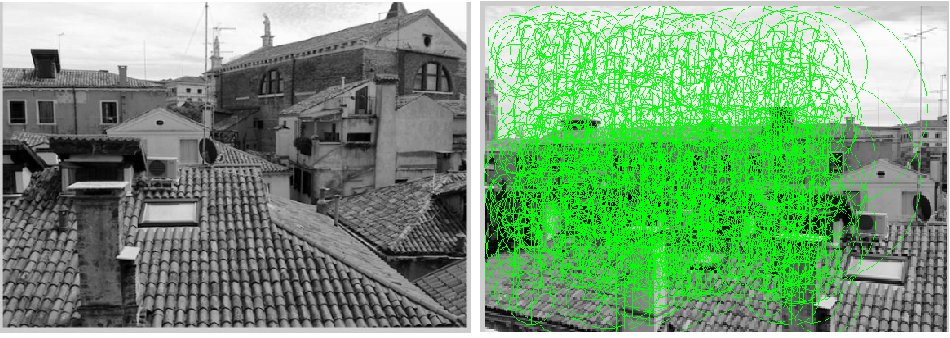
\includegraphics[,scale=0.6]{./img/sift.png}
		\caption{Пример ключевых точек SIFT.}  
		\label{1-sift}
\end{figure}

\textbf{Метод SURF}

Для ускорения обработки был предложен дескриптор SURF, который использует интегральные изображения и приближённые детерминанты матрицы Гессе для быстрого обнаружения ключевых точек \cite{18}. SURF формирует 64-мерный или 128-мерный дескриптор на основе распределения гауссовых вейвлет-ответов в окрестности точки.

Ниже, на рисунке \ref{1-surf}, представлен пример ключевых точек SURF.

\captionsetup{justification=centering,singlelinecheck=off}
\begin{figure}[h!]
	\centering
		\includegraphics[,scale=1.0]{./img/surf.png}
		\caption{Пример ключевых точек SURF.}  
		\label{1-surf}
\end{figure}

По сравнению с SIFT, SURF работает в несколько раз быстрее при сопоставимой точности для большинства типов фальсификаций копирование-вставка. Однако SURF уступает SIFT при сильных аффинных искажениях и при низкой освещённости. В задачах обнаружения фальсификаций SURF часто выбирают для систем реального времени или для обработки больших массивов изображений, когда время критичнее максимальной точности\cite{19}.

Основное ускорение SURF достигается за счёт использования интегральных изображений, позволяющих вычислять сумму пикселей в произвольном прямоугольнике, независимо от его размера. Это делает возможным быстрое вычисление детерминанта матрицы Гессе с использованием приближённых бокс-фильтров вместо гауссовых свёрток. Детектор SURF использует детерминант матрицы Гессе для локализации точек интереса, где значение детерминанта достигает максимума. Дескриптор SURF вычисляется путём суммирования откликов гауссовых вейвлетов (фильтров Хаара) в окрестности точки, ориентированных согласно основной ориентации, которая определяется по гистограмме откликов Хаара в круговой области. 64-мерный вариант дескриптора содержит значения суммы и суммы абсолютных значений откликов Хаара по четырём направлениям для каждого из 4×4 субрегионов, что даёт 4×4×4 = 64 измерения. 128-мерный вариант дополнительно разделяет отклики по знаку, что увеличивает различительную способность за счёт учёта не только величины, но и направления градиента.

На практике разница в скорости становится заметной уже на изображениях размером 1024×768 пикселей: SURF обрабатывает такое изображение за 0.2–0.3 секунды, тогда как SIFT – за 1.5–2 секунды \cite{18}. Для мобильных приложений или веб-сервисов, где требуется ответ менее чем за секунду, SURF оказывается предпочтительнее. Однако при работе с низкоконтрастными изображениями SURF генерирует значительно меньше устойчивых ключевых точек, чем SIFT, что может привести к пропуску фальсификации \cite{11111}. 

Важной особенностью SURF является возможность выбора размера дескриптора: 64-мерный вариант быстрее в сравнении, но даёт больше ложных совпадений на текстурированных фонах. 128-мерный вариант работает медленнее, но обеспечивает точность, близкую к SIFT. При реализации систем обнаружения копирование-вставка часто используют 64-мерный SURF на первом этапе грубого поиска, а затем верифицируют подозрительные кластеры с помощью более точного SIFT-дескриптора. Такой гибридный подход позволяет достичь компромисса между скоростью и точностью \cite{19}. 

Снижение количества генерируемых ключевых точек на низкоконтрастных изображениях обусловлено тем, что детектор SURF использует фиксированный порог для детерминанта матрицы Гессе. На изображениях с низким динамическим диапазоном значения детерминанта могут не достигать этого порога, даже если визуально присутствуют характерные особенности. Это приводит к тому, что при работе с тёмными или плохо освещёнными изображениями SURF может не обнаружить дублированных областей, которые SIFT с его адаптивным механизмом выделения экстремумов всё ещё способен распознать. С другой стороны, на изображениях с высоким уровнем текстуры SURF генерирует множество точек, что увеличивает вероятность ложных срабатываний. Поэтому выбор между SIFT и SURF в значительной степени зависит от условий съёмки исходных изображений и требуемой скорости обработки.

Кроме того, SURF, как и SIFT, не способен обнаружить фальсификации, если дублированная область была предварительно размыта или к ней применили нелинейную фильтрацию. Даже лёгкое медианное размытие с окном 3×3 снижает количество правильных совпадений на 60–70\%. Поэтому при разработке системы, устойчивой к постобработке, дескрипторные методы рекомендуется дополнять фильтрацией высоких частот или анализом остаточных шумов.

Природа этой уязвимости связана с тем, что ключевые точки по своей сути являются экстремумами в градиентном поле. Размытие (как линейное, так и медианное) сглаживает высокочастотные составляющие изображения, уменьшая амплитуду градиентов и смещая положение экстремумов. В результате многие точки либо исчезают, либо их дескрипторы меняются настолько, что расстояние до соответствующей точки в дублированной области превышает допустимый порог. Особенно критичным является медианное размытие, которое не только сглаживает, но и создаёт ступенчатые артефакты на границах объектов, что дополнительно искажает гистограммы градиентов. Для преодоления этого ограничения исследователи предлагают применять предварительную обработку изображения, направленную на восстановление высокочастотных компонент, например, с помощью фильтрации в частотной области, усиления контуров или вейвлет-декомпозиции с подавлением низкочастотных составляющих. Однако такие методы требуют аккуратной настройки параметров, чтобы не внести дополнительные артефакты, которые сами по себе могут быть ошибочно интерпретированы как признаки фальсификации.

\textbf{Ограничения методов на основе ключевых точек}

При применении SIFT/SURF для анализа больших коллекций изображений важно задать минимальное количество ключевых точек, необходимое для принятия решения о наличии копирование-вставки. Опыт показывает, что порог в 8–12 совпадающих точек достаточно надёжно отсеивает случайные совпадения, но может пропускать подделки с очень маленькими скопированными фрагментами \cite{15}. Для обнаружения мелких вставок порог снижают до 4–5 точек, но при этом резко возрастает число ложных срабатываний на текстурированных фонах. В таких случаях помогает дополнительная проверка формы области: если найденный кластер точек вытянут вдоль границы объекта, вероятность реальной подделки выше, чем для компактного кластера.

Ещё одной практической проблемой является то, что алгоритмы кластеризации требуют задания максимального евклидова расстояния между дескрипторами в пространстве признаков. Это расстояние зависит от степени сжатия изображения и уровня шума. Для JPEG с качеством 95\% разумное пороговое значение составляет 0.6–0.7, а для качества 70\% порог приходится увеличивать до 0.8–0.9, что ведёт к росту ложных совпадений. Поэтому перед анализом рекомендуется оценивать коэффициент качества JPEG и адаптивно подбирать порог. В автоматизированных системах это можно реализовать через предварительный анализ DCT-гистограммы.

Наконец, отметить, что SIFT и SURF дают наилучшие результаты при разрешении входного изображения не ниже 640×480 пикселей. При меньшем разрешении количество ключевых точек падает настолько, что даже очевидные copy-move подделки могут остаться незамеченными. Для низкоразрешенных изображений более эффективными оказываются методы, основанные на блочном сравнении без ключевых точек, либо сверточные нейронные сети, работающие непосредственно с пикселями \cite{11112}.

Зависимость от разрешения объясняется тем, что масштабная пирамида SIFT имеет конечное число октав, и при малых размерах изображения на верхних уровнях пирамиды фактически отсутствует достаточное количество пикселей для выделения устойчивых экстремумов. Кроме того, на изображениях с низким разрешением сглаживание, применяемое при построении масштабного пространства, захватывает значительную часть полезного сигнала, что приводит к потере мелких деталей, на которых часто строятся характерные ключевые точки. Это делает дескрипторные методы неприменимыми для обнаружения фальсификаций на изображениях, поступающих из социальных сетей, где многие платформы автоматически сжимают и уменьшают разрешение загружаемых фотографий. В таких сценариях нейросетевые подходы, работающие на уровне пикселей и не требующие явного детектирования ключевых точек, демонстрируют значительно более высокую эффективность, что подтверждает целесообразность разработки гибридных систем, сочетающих быстрые дескрипторные методы для первичного анализа и глубинные нейронные сети для верификации на подозрительных областях.

\subsection{Метод на основе сверточной нейронной сети}

Методы обнаружения фальсифицированных фрагментов на основе свёрточных нейронных сетей (CNN) в последние годы заняли доминирующее положение в области компьютерной криминалистики изображений. В отличие от классических подходов (анализ целостности или поиск ключевых точек), которые требуют ручного проектирования признаков, CNN автоматически извлекают иерархические представления из данных, обучаясь различать подлинные и поддельные области на больших размеченных наборах. Способность сетей выявлять сложные статистические аномалии, невидимые для традиционных детекторов, обусловила их широкое применение для выявления вставки объектов, копирования-вставки и так далее \cite{22}.

Фундаментальное преимущество сверточных нейронных сетей заключается в их способности обучаться представлениям данных непосредственно из пиксельных значений, без необходимости вручную определять, какие именно признаки являются информативными для задачи обнаружения. В процессе обучения сеть автоматически формирует иерархию признаков: на ранних слоях выделяются простые локальные структуры (края, углы, текстуры), на средних — более сложные комбинации (формы, паттерны), а на глубоких — семантически значимые концепции (объекты, сцены, глобальные корреляции). Для задачи обнаружения фальсификаций это означает, что сеть способна одновременно учитывать как низкоуровневые артефакты (нарушения шумовой структуры, несоответствия в частотных характеристиках), так и высокоуровневые несоответствия (неправильная перспектива, несоответствие освещения, аномалии в текстуре). Такая многоуровневая обработка делает CNN принципиально более гибкими и мощными по сравнению с методами, использующими фиксированные, заранее определённые признаки.

Первые работы по применению CNN для обнаружения подделок использовали простую архитектуру с несколькими свёрточными и полносвязными слоями, работавшую на входных изображениях фиксированного малого размера (например, 64×64 или 128×128). Такие сети классифицировали небольшие патчи как подлинные или поддельные, после чего для локализации фальсификации применялся скользящий оконный метод \cite{24}. Хотя этот подход демонстрировал приемлемую точность на сбалансированных датасетах, он был вычислительно затратным и давал высокую долю ложноположительных срабатываний на границах объектов. Кроме того, сети, обученные на патчах, часто запоминали артефакты конкретного типа фальсификации и плохо обобщались на другие типы фальсификаций.

Патчевый подход имеет несколько фундаментальных ограничений, которые делают его непригодным для практического применения в реальных условиях. Во-первых, фиксированный размер патча означает, что сеть не может использовать контекстную информацию за пределами этого окна, что особенно критично при обнаружении вставок, где соответствие между вставленным объектом и окружающим фоном является важным признаком. Во-вторых, скользящее окно с шагом, меньшим размера патча, приводит к многократной обработке одних и тех же пикселей, что резко увеличивает вычислительную сложность — для изображения 1024×1024 с патчем 64×64 потребуется выполнить более 200 тысяч классификаций. В-третьих, решение о классификации каждого патча принимается независимо, без учёта пространственной согласованности соседних областей, что приводит к «шумным» маскам с разрозненными ложными срабатываниями. Наконец, сети, обученные на патчах, склонны к переобучению под конкретные артефакты, присутствующие в обучающей выборке (например, определённый тип JPEG-артефактов или характерные границы вставки), и теряют эффективность при появлении новых типов фальсификаций или при изменении условий съёмки.

Прорывом стало появление полностью свёрточных сетей (FCN --- Fully Convolutional Networks), которые на входе принимают изображение произвольного размера и на выходе выдают карту локализации той же пространственной размерности. Архитектура типа U-Net (симметричный энкодер-декодер с пропускными соединениями) стала стандартом для пиксельной сегментации подделанных областей \cite{23}. Энкодер последовательно уменьшает пространственное разрешение, извлекая всё более абстрактные признаки, а декодер восстанавливает детализацию и формирует маску подделки. Пропускные соединения позволяют сохранить мелкие гранулярные признаки, которые иначе теряются при многократном субдискретизации \cite{26}. 

Архитектура энкодер-декодер (U-Net) с пропускными соединениями решает сразу несколько ключевых проблем, характерных для патчевых подходов. Энкодер, состоящий из последовательности свёрточных слоёв с операциями понижения разрешения (субдискретизации), формирует компактное представление изображения, содержащее информацию о глобальном контексте и семантике сцены. Это позволяет сети понимать, какие объекты и структуры являются «нормальными» для данного типа изображения, и выявлять глобальные несоответствия. Декодер, напротив, последовательно восстанавливает пространственное разрешение, используя информацию из энкодера для точной локализации границ подделки. Пропускные соединения между соответствующими уровнями энкодера и декодера обеспечивают передачу детальной пространственной информации, которая была бы потеряна при многократной субдискретизации. В результате сеть способна одновременно учитывать как глобальный контекст (для понимания того, что вставка семантически не соответствует сцене), так и локальные детали (для точного выделения границ вставленного объекта). Такая архитектура является наиболее эффективной для задач сегментации, где требуется точное попиксельное выделение областей интереса.

Ниже, на рисунке \ref{1-unet}, представлена архитектура U-Net.

\captionsetup{justification=centering,singlelinecheck=off}
\begin{figure}[h!]
	\centering
		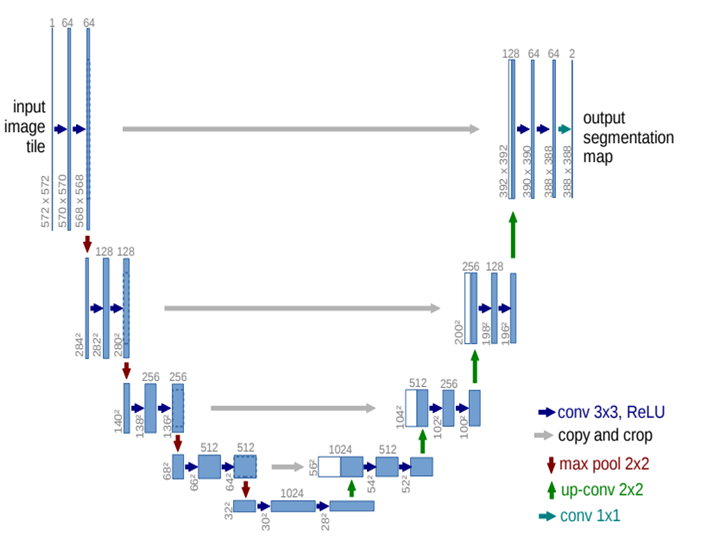
\includegraphics[,scale=0.6]{./img/unet.png}
		\caption{Архитектура U-Net.}  
		\label{1-unet}
\end{figure}

Важным направлением является использование не RGB-изображений в качестве входа, а так называемых остаточных карт, полученных вычитанием из исходного изображения его сглаженной версии. Такой подход подавляет семантическое содержание и усиливает следы камеры и постобработки. Сеть, обученная на остатках, оказывается более устойчивой к сжатию JPEG и изменениям контента, поскольку вынуждена фокусироваться на статистических аномалиях, а не на форме объектов \cite{25}.

Для борьбы с разнообразием типов подделок и усложняющих обработок исследователи разрабатывают многозадачные и многомасштабные архитектуры. Один из подходов – использование параллельных ветвей сети, работающих на разных масштабах, с последующим объединением карт признаков. Другой – применение механизмов внимания, которые позволяют сети динамически взвешивать важность различных пространственных областей и каналов признаков.

Одной из ключевых проблем CNN-методов является их чувствительность к различиям между обучающими и тестовыми датасетами. Сеть, обученная на изображениях с одними камерами и степенями сжатия, может резко терять точность при тестировании на других. Для повышения обобщающей способности применяют методы аугментации, где сеть обучается одновременно на подлинных и сгенерированных подделках, устойчивых к детектированию. В последнее время активно развиваются методы адаптации признаков, которые выравнивают распределения признаков из разных доменов с помощью градиентного реверса слоя или вариационных автоэнкодеров.

Несмотря на высокие показатели качества, CNN-методы имеют и недостатки. Во-первых, они требуют больших размеченных наборов данных с пиксельной маской подделки, создание которых трудоёмко. Во-вторых, многие модели «чёрный ящик»: сложно интерпретировать, на каком именно основании сеть отнесла область к подделанной. В-третьих, вычислительные затраты на обучение глубоких сетей высоки, и для работы в реальном времени часто требуется GPU-ускорение \cite{2}.

\section{Сравнительный анализ методов фальсифицированного фрагмента на изображении}

\subsection{Обоснование критериев сравнения методов}

Для объективного и всестороннего сопоставления различных методов обнаружения фальсифицированного фрагмента на изображении необходимо определить систему критериев, отражающих как точность детекции, так и пригодность метода для практического применения в реальных условиях. Выбор критериев должен основываться на требованиях, предъявляемых к современным системам цифровой криминалистики, а также на особенностях задач, возникающих при анализе медиаконтента в социальных сетях, новостных агрегаторах и системах информационной безопасности. В настоящей работе предлагается использовать пять основных критериев, каждый из которых характеризует определённый аспект эффективности метода.

Первым и наиболее важным критерием является точность локализации подделанного фрагмента. В отличие от бинарной классификации, где требуется лишь определить факт наличия фальсификации, задача локализации требует указать точные границы изменённой области на пиксельном уровне. Высокое значение точности локализации свидетельствует о том, что метод способен не только обнаружить факт вмешательства, но и точно выделить форму вставленного объекта, что критически важно для последующего анализа и использования результатов в качестве доказательной базы. Оценка точности локализации обычно производится с использованием таких метрик, как индекс пересечения над объединением и F1-мера, которые учитывают как полноту обнаружения поддельных пикселей, так и долю ложноположительных срабатываний. Следует отметить, что высокая точность бинарной классификации ещё не гарантирует точной локализации, поэтому данные метрики должны рассчитываться отдельно для каждой тестовой выборки.

Второй критерий — устойчивость к постобработке изображения. В реальных условиях фальсифицированное изображение почти всегда подвергается сжатию с потерями (особенно в формате JPEG), изменению размера, добавлению шума или применению различных фильтров. Злоумышленник может намеренно применять такие операции для маскировки следов фальсификации, стремясь сделать их невидимыми для автоматических детекторов. Поэтому метод должен сохранять высокую точность обнаружения при различных степенях сжатия JPEG, при изменении разрешения и при добавлении различных видов шума. Устойчивость к постобработке является одним из ключевых требований к практическим системам, поскольку в интернете подавляющее большинство изображений хранится и передаётся в сжатом виде. Сравнение методов по данному критерию должно проводиться при разных коэффициентах качества JPEG и при различных типах и уровнях постобработки, что позволяет оценить робастность каждого подхода.

Третий критерий — обобщающая способность на неизвестных типах фальсификации и датасетах. Метод не должен «переобучаться» под конкретный набор данных или под конкретный тип манипуляций. В идеале обученная модель должна корректно работать на изображениях, полученных из других источников, с другими камерами, с другими типами сжатия и с другими видами фальсификаций. Для оценки обобщающей способности применяется кросс-валидация на различных датасетах: обучение проводится на одном наборе данных, а тестирование — на другом. Этот критерий особенно важен для нейросетевых методов, которые в силу своей высокой ёмкости могут запоминать специфические артефакты обучающей выборки и терять эффективность при переходе к новым данным.

\subsection{Таблица сравнения методов}

На основе обоснованных в п. 1.3.1 критериев (точность, робастность к постобработке и обобщающая способность) проведём сравнительный анализ трёх основных классов методов обнаружения фальсифицированного фрагмента: аналитических методов целостности, дескрипторных методов на основе ключевых точек и методов на основе свёрточных нейронных сетей (включая их расширения с вниманием и адаптацией признаков). Для каждого критерия используется качественная шкала: «высокая», «средняя», «низкая», а также уточняющие комментарии. Результаты сведены в таблицу \ref{tab:compare}.

\begin{table}[H]
	\centering
	\caption{Сравнительная таблица методов}\label{tab:compare}
	\begin{tabular}{|p{3.7cm}|p{3.6cm}|p{3.6cm}|p{3.6cm}|}
		\hline
        \textit{Метод} & \textit{Точность}  & \textit{Устойчивость к постобработке} & \textit{Обобщающая способность} \\ \hline
        Методы на основе анализа целостности изображений & Низкая/Средняя & Низкая & Низкая \\ \hline
		Методы на основе поиска ключевых точек & Средняя & Средняя & Низкая \\ \hline
		Однопоточная сверточная нейронная сеть & Средняя/Высокая & Средняя & Средняя \\ \hline
		Многопоточная сверточная нейронная сеть & Высокая & Средняя/Высокая & Средняя/Высокая \\ \hline
	\end{tabular}
\end{table}

На основе данных таблицы 1.1 можно сделать следующие выводы. 

Методы на основе анализа целостности изображений обладают неоспоримым преимуществом в независимости от обучающих данных. Однако их точность и робастность к постобработке остаются низкими, особенно при сжатии JPEG ниже 80% качества, при изменении размера или при применении нелинейной фильтрации. Кроме того, локализация фальсификации этими методами часто осуществляется лишь на уровне оценки «подозрительности» отдельных блоков, что даёт лишь грубую оценку области вмешательства. Поэтому данные методы рекомендуются в первую очередь для задач, где интерпретируемость и юридическая достоверность важнее максимальной точности, а также в качестве вспомогательного инструмента для первичной фильтрации подозрительных изображений.

Методы на основе поиска ключевых точек (SIFT, SURF) показывают высокую точность локализации фальсификации типа «копирование-вставка» (copy-move), поскольку способны выявлять повторяющиеся фрагменты даже после геометрических преобразований. Это делает их наиболее эффективным инструментом для обнаружения дублирования объектов внутри одного изображения. Их главные недостатки — непригодность для выявления других типов фальсификаций (splicing, inpainting), а также вычислительная сложность, ограничивающая применение на высокоразрешенных изображениях (свыше 10 мегапикселей) и в системах реального времени. Кроме того, устойчивость к постобработке у этих методов ограничена: даже умеренное сжатие JPEG или медианная фильтрация могут существенно снизить количество детектируемых ключевых точек и, следовательно, точность обнаружения. Несмотря на это, методы на основе ключевых точек остаются важным инструментом в арсенале специалистов по компьютерной криминалистике, особенно когда требуется быстро проверить изображение на наличие признаков копирования.

Нейросетевые методы на основе свёрточных нейронных сетей демонстрируют наилучшие показатели по точности локализации и робастности к постобработке, а также способны обнаруживать широкий спектр подделок — от copy-move до deepfake и полностью синтетических изображений. Это обусловлено способностью CNN автоматически извлекать иерархические признаки из данных и адаптироваться к разнообразным типам манипуляций. Особенно высокие результаты достигаются при использовании двухпоточных архитектур, которые разделяют анализ низкоуровневых шумовых артефактов и высокоуровневого семантического содержания, а также при применении механизмов внимания и слоёв адаптации признаков для согласования признаков из разных доменов. Однако нейросетевые методы имеют и существенные недостатки: низкая интерпретируемость («чёрный ящик»), высокая зависимость от размера и качества обучающей выборки, а также значительные вычислительные затраты на обучение и инференс. Кроме того, нейросетевые подходы чувствительны к различиям между обучающими и тестовыми датасетами, что требует применения тщательной аугментации и, в некоторых случаях, доменной адаптации.

Таким образом, проведённый сравнительный анализ позволяет заключить, что для разработки практического метода обнаружения фальсифицированных фрагментов, способного работать в реальных условиях с различными типами подделок и постобработок, наиболее перспективным является подход на основе двухпоточной свёрточной нейронной сети с механизмами внимания и адаптации признаков. Этот подход сочетает высокую точность локализации, хорошую обобщающую способность и устойчивость к сжатию JPEG, что делает его наиболее подходящим для решения поставленной задачи. В то же время необходимо уделять внимание повышению интерпретируемости и снижению вычислительной сложности, что может быть достигнуто путём оптимизации архитектуры и использования методов визуализации активаций.

\section{Формализованная постановка задачи}

В настоящей работе проектируется метод обнаружения фальсифицированного фрагмента на изображении с помощью свёрточной нейронной сети, а именно --- двухпоточной архитектуры с слоями вниманий и адаптацией признаков. Набор данных для обучения должен быть подготовлен --- должно быть установлен уникальное соответствие между входным изображением и бинарной маской. Набор данных должен быть предварительно обработан и извлечены признаки. Обученная модель используется для распознавания границ фальсифицированного фрагмента и выдачи маски локализации.

Ниже, на рисунке \ref{1-problem}, представлена IDEF0-диаграмма нулевого уровня.

\captionsetup{justification=centering,singlelinecheck=off}
\begin{figure}[h!]
	\centering
		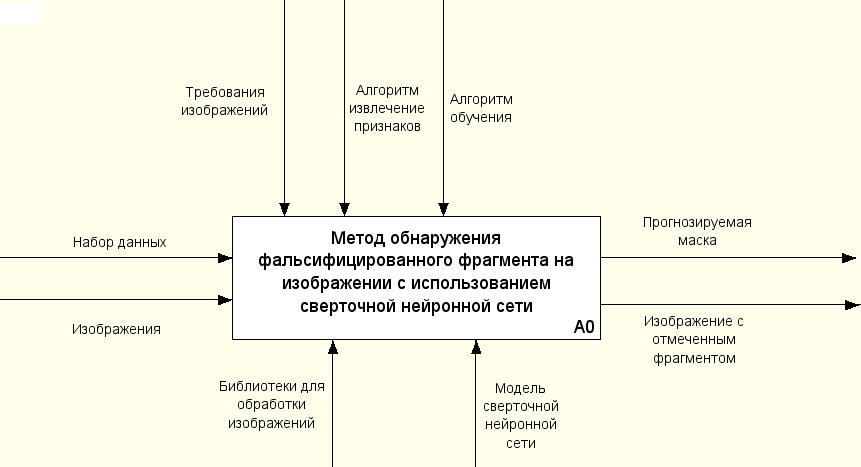
\includegraphics[,scale=0.7]{./img/idef0.png}
		\caption{IDEF0-диаграмма нулевого уровня}  
		\label{1-problem}
\end{figure}
\newpage

\section*{Вывод}
% \addcontentsline{toc}{section}{Вывод}
% В данном разделе был проведен анализ предметной области. Был проведен обзор методов обнаружения фальсификаций на изображения и их сравнение. Была представлена формализованная постановка задачи в виде IDEF0-диаграммы.

В данном разделе был проведен анализ предметной области. Также был проведен обзор методов обнаружения фальсификаций в изображении. Были сформулировали критерии их сраванения и проведен сравнительный анализ рассмотренных методов. Также в этом разделе была представлена формализованная постановка задачи в виде IDEF0-диаграммы.

